\section{Scheduler Component Architecture (SCA)}
%\chapter{Scheduler Component Architecture (SCA)}
\label{sect:sched_comp_study}
This is a major part of the research - define what are the basic components required to build a variety of observing schedulers

\subsection{Intro and rational}
Describe pricniple behind design of initial deploy system (IDS)- what was learnt from IDS and incorporated into SCA - then describe individual components from base comps upward (xm/p2m/am/hm to Despatcher).

Describe how the scheduler is implemented and how it fits in and interacts with other systems. In this bit also need to justify why it is what it is, how well it works (or not) - NO later... and how it relates to the other implementations discussed in the literature (above). or does this go into appendix - need some detail to justify reason for experiments in first place!

overall architecture
This can be on several levels -
Communications - how the scheduler interacts with executor and updater - the exec loop. diagrams
Detailed internal operation of engine. an algorithm or timing diag plus component diag.



\subsection{SCA Components}

\subsubsection{Environmental Prediction Model - ($E$)}
Models the environment the scope exists in. Uncertain, should provide current and possibly predictive estimates of the variables. Predictive useful to fold in to likeliness indicator of 'availability and utility' of future observing periods. Scheduler would like to be able to look ahead and decide if its best to do X now or wait for half an hour when seeing is likely to be better
Some Variables:-
seeing - photometricity/extinction \cite{lapalma31,lapalma115} - sky brightness \cite{krisciunas91brightness,krisciunas97optical} - cloud/dust - temperature - bad weather, rain,wind,humidity = scope out-of-action.

How do we get this stuff into the EM and how do we do prediction - is it worth it? what lookahead horizon? - there are a number of papers on this  \cite{aussem94dynamical,aussem94fuzzy,sarazin97automated,aussem02online,racine96temporal} also some useful stuff on VLT weather station), used neural nets with various time averaged meteo indicators - results uninspiring not much better than climatological stats. 

ING weather stuff and LT data. Dont need technical details of how this is processed by RCS or how it is measured. 

A number of standard models have been set up for use in the simulations.

\begin{description}
\item[ $E_{Fp}$] Seeing is kept constant in the \emph{poor} state.
\item[ $E_{Fa}$] Seeing is kept constant in the \emph{average} state.
\item[ $E_{Fx}$] Seeing is kept constant in the \emph{excellent} state.
\item[ $E_{Ra}$] Random using annual (climatological) distribution. 
\item[ $E_{Rs}$] Random using seasonal distribution.
\item[ $E_{N(<date>)}$] Actual seeing history recorded from a given night. 
\item[ $E_{R_{uvw}}$] Random using supplied values for probability distribution between Poor (u), Average (v) and Excellent (w) seeing.
\item[ $E_{S_{<ID>}}$] Scenario-based with specified scenario ID.
\end{description}

Additional (simulation) models proposed which use actual environmental scenario from simulation with varying degrees of accuracy over specified look-ahead periods.

\subsubsection{Weather prediction model -($W$)} 
This predicts the future weather. 

\subsubsection{Execution timing ($X$) and feasibility ($\Phi$) models}
These are the scheduler's models of the function of the executor (RCS or simulator or whatever). They provide information about the feasibility and resource consumption of groups of observations. Specifically we need to know 'can group x be done at t ?' and 'how long will it take to do group x ?' Scheduler may want this information broken down e.g. 'how much of that time is just slewing or acquiring ?' Execution is a stochastic process - the effects of parallel execution of the decomposed tasks and various heuristics used by the executor along with genuine uncertainty in individual execution times of sub tasks (e.g. time to acquire with A/G, time for filter change going one way or other, mysterious internal calibration within instruments). Important this estimate is good - over-estimate could lead to a potential candidate being rejected for no good reason, under-estimate could lead to selection of an unsuitable candidate.

Describe the various events that feed into this model - rcs/tcs/ics info is needed plus when feasible external timing constraints
Describe the various items to take into account (number of slews/rotator shifts, offsets (mosaic or requested by instrument), reconfiguration (including focus offsets etc)). also acquisition autoguiding, backoffs and retries - how frequent)? Complexity of executor's task decomposition.

\begin{itemize}
\item slew rate in each axis, when target changes, rot mode or angle changes, rot CP solution changes
\item instrument filter defocus
\item fold mirror move/deploy when inst changes
\item instrument config change (filter wheel, grating etc)
\item instrument calibration before/after image, lamp calibs
\item configuration of acquisition inst when required
\item acquisition by acquisition instrument onto spectrograph slit
\item autoguider acquisition
\item aperture offsets
\item readout time (per instrument) also depends on binning and windowing
\item data write-to-disc time (per instrument)
\item recovery and retry time delays
\end{itemize}

There is a need to distinguish between the model used by the scheduler to work out the likely execution times and the stochastic model used by the executor (simulation control application) to decide how long the group will actually take. 

Some notes about combining uniform random distributions (assume each variable param is uniform random) - use poisson or binomial distibution - some simulations with an example group.

some examples of xms - can we get some real data ? needs extra embedded instrumentation and a way to store e.g. mysql on occ.can we just pull from stored history data. TBD check hist items for some frequent group. NO just the nominal time is stored though RCS knows it anyway.


\subsection{(External) Timing constraint calculator } 
Or a better name for this (TCWC). This provides information about when the executor will be available for scheduled operations - i.e. when it wont be down for engineering, realtime, calibration or any other downtime - even daytime?
How long should we provide this info for?
1 night ahead seems reasonable esp. for dynamic despatch BUT say we know the scope is hors d'action for next 2 nights and we have a group which should be executed once either tonight or next 2 nights then expires - we must do it tonight if at all possible and if the cost of not doing it at all is high enough. Scheduler may want to fold in this certain knowledge intop a predictive 'look-ahead' attempt to decide when the telescope will be usable along with the various sources of uncertain knowledge e.g. from env model predictions or from measures of expected utility for various observing strategies (DM:proposal-specific).

This needs details of 2 seperate modules:- ETCC and TCWC which fulfil quite different functions.


\subsubsection{Spatial constraints model} 
- do we need this amount of detail ? basically which bits of sky we cant see. This really doesnt apply to LT - could do if dome is half-closed for some reason.

\subsubsection{Phase2 model - ($P$)} 

This is the information entered by the observers or on their behalf by automated agents which describes the content and constraints of the observing programs - i.e what to do and when. The information can be broken into the following categories:-

\begin{itemize}
\item Observation specifications - details of the observations; target selection, acquisition and tracking information, instrument selection and configuration, number and length of exposures, mosaic/dither offset patterns.
\item Timing constraints - when and how often to perform groups of observations.
\item Observing constraints- limitations on the conditions under which the observations may be taken.
\item Observing preferences - quantification of the observer's tradeoffs between competing effects in determining the value of performing observations under particular conditions or at specific times.
\item Quality requirements - limitations on the amount, regularity and quality of data taken - is this neccessary?
\end{itemize}



\subsubsection{History model - ($H$)}
The history model (H) represents the record of execution histories of groups from the phase2 model. For flexibly scheduled single execution groups this is just the date/time it was executed. For repeating groups it represents all of the times the group has previously been executed along with relevant execution statistics. 

\subsubsection{Accounting model - ($A$)}
The allocation and use of resources by groups, proposals and TAGs is provided through the accounting model (A). The simple accounting model provides access only to the accumulated balance of the various accounts, a more advanced accounting model envisoned for the future deployed system will allow the history of transactions to be followed as an audit trail.

\subsubsection{Cost accounting model - ($C$)}
When observers prepare their proposals to go before the TAG for time and resource allocation the cost or charging model (C) is  used to calculate the amount of time the groups \emph{should} take to execute. The standard figures for slewing, acquisition, readout and instrument reconfiguration defined in the charging model are published on the telescope website for observers to calculate their resource requirements and these same values are used to calculate the nominal cost of performing a group. In reality a group may take more or less time than this but this is the resource usage which is charged to the relevant account. It is expected that this model will be integrated into a future user GUI by way of a webservice endpoint.

\subsection{Scheduling engine}

\subsubsection{Selection Heuristic - ($\zeta$)}
That which makes the selection from the supplied metrics or scored metrics (different, one has score calculated other just the unweighted metric vector).

\subsubsection{Scoring model - ($S$)}
This is what works out the score for a group. Mention differing HSM metrics and combining weights- or can define Metric generator ($M$) and metric vector $\mathbf{m}$ which can be pushed to candidate selector $\zeta(\mathbf{m}$).



\subsection{Heuristic Scoring metrics (HSM)}

These are the metrics actually used by the scheduler to rank the list of potential observation group candidates to do next from the pool of available groups. 

Some of these metrics are peculiar to despatch shchedulers, others are more generally applicable.

\begin{itemize}
 
\item Height metric $f_h$ simply measures the elevation of the group's target at the time of potential observation. Variations on this metric can inlcude taking the mean or peak elevation over the duration of the group. If a group has multiple targets various averages can be used such as taking mean elevation of each target at some point in the execution. More complex averages could take into account the actual times at which each target will be observed. 
 
\item Airmass metric $f_{air}$ is similar to $f_h$ except that the airmass is used rather than elevation thus taking into account the nonlinear nature of the relationship between sky-quality and elevation.

\item Transit metric $f_{trans}$ is an attempt to take into account the unfair advantage provided by the two previous metrics $f_h$ and $f_{air}$. These force a bias towards targets whose declination is close to the latitude of the observatory. This metric measures the quality of observing at a given time by taking the current target elevation as a fraction of its \emph{best} elevation. This is generally taken as its transit elevation which can be calculated easily. For groups which do not transit during the feasibility window and in particular for groups with very short feasibility windows this may still be somewhat unfair as the transit elevation may not be remotely achievable in that window.

\item Optimal elevation $f_{oh}$ and optimal airmass $f_{oa}$ metrics attempt to redress this problem by taking the ratio of current elevation to \emph{best possible} elevation (or airmass) in the group's feasibility window. 

\item Slew metric $f_{slew}$ attempts to penalize groups for which a long axis slew (including rotator) from the current telescope position is required. This can prove very difficult to calculate as it requires the scheduler to predict the way the executor will choose rotation angles - the recently introduced cardinal pointing (CP) regime on the LT to handle the problem of coolant pipes in the wrap makes this particularly difficult to determine.

\item Sky condition matching metrics $f_{see}$ (also $f_{phot}$ and $f_{sky}$) is designed to match a group's sky condition requirements to the actual (or predicted) conditions at the time of execution. This is intended to ensure that groups which do not require particularly good conditions do not take an excessive share of good conditions.
 
\item Lunar condition matching metric $f_{moon}$ is similar to the above but attempts to prevent groups which can use \emph{bright} time from taking an excessive shar of \emph{dark} time.

\item Priority metric $f_p$ is designed to ensure that groups of higher scientific priority get a better share of time. 

\item Resource allocation metric $f_{a}$ measures the use of various resources by a group or its containing proposal. This is typically the use of time from the proposal's total semester allowance. It can be used either to help distribute time fairly between proposals or to force completion of proposals which have already been started.

\item Demand metric $f_{dmd}$ uses the group's demand for time as an indication of the urgency of performing the group (see XXX). The idea behind this is to select the groups which have the most critical requirment for a given time period.

\item Urgency metric $f_{urg}$ is similar to the demand metric but measures the number of additional chances (in terms of alternative nights on which the group \emph{could} be observed if not tonight.

\item Yield tracking metric $f_{yt}$ tracking deficit in data product yield - needs past and future yield estimates and yield to-date to allow effect of any deficit to be deduced.

\end{itemize}
 
For each of these metrics there are various possibilities for weighting.

\begin{itemize}
\item No special weighting.
\item Groups \emph{expected} execution time is used to weight the metric.
\item The group's total exposure time is used as a weighting factor.
\item Group's priority (or some function of this) is used to scale the metric.
\end{itemize}



\subsection{Simulation framework}

Here I discuss the additional comonents required to implement a simulation framework with which to test various schedulers. Need to mention simple model used with basic DS and short LAS but additional complexity when scheduler runs in parallel with executor but with realtime running costs.


Need a framework to run the scheduler in. Currently looking at running scheduling engine continuously at some predefined rate with additional planning layers running at slower rate - how the Scheduler's run-rate (better name?) is chosen is dependant on the rate at which the ODB changes - if we run every 30 minutes and ODB changes \emph{significantly} on that timescale we will either miss opportunities or do unnecessary (unprofitable) work - both lead to reduced cumulative reward. Consequently the need for some sort of feedback from the ODB (Phase2Model) may be needed - suggests some sort of {\tt Phase2ModelUpdateListener} interface that the SE can register as. This would most likely just have a simple implementation like a method {\tt phase2ModelUpdated(Phase2Event pe)}. 

How do we decide when a \emph{significant} change has occurred ? -  Suggest each event type has some sort of weighting associated and we just increment a score as the events come in - maybe need to consider if the event's target is involved in the current schedule as part of the assessment. When a threshhold is exceeded this could prompt a rerun of the scheduler. We dont want the scheduler re-running each time an ODB change occurs - this will lead to reduced \emph{effective horizon} and reduced profit. Opportunity here for some learning - i.e. measure the rate of change of the ODB and set the scheduler run rate dependant on this - {\bf adaptive run rate} (better acronym please).

Because the (simulation) scheduler will be running faster than realtime (i.e. it will execute in realtime but gaps will be speeded up) and the executor (simulator) will also be running (in parallel) in model-time we need some way to synchronize the two - this suggests the need for a discrete event queue to control the model clock (i.e. {\tt DiscreteEventSimulationTimeModel}. This had {\bf not} previously been considered neccessary as the scheduler was expected to run on request from the Executor. This turns out to be a bit of a bugger to implement - not difficult for a simulated SE and Executor but I am exepecting to use the \emph{real} SE here. I would expect to have it run using some sort of polling loop i.e. something like:-

\begin{algorithm}
\label{alg:schedrealrun}
\begin{algorithmic}
  \WHILE{true}
    \STATE run scheduler
    \STATE sleep $\delta$t 
  \ENDWHILE
\end{algorithmic}
\caption{Realtime scheduler run cycle}
\end{algorithm}

To allow the \emph{real} SE to be used in simulation, in addition to being able to switch the {\tt TimeModel} from {\tt RealTimeModel} to {\tt SimulatedTimeModel} which can be set by the franework, it will be neccessary to privide simulated clock to inject events/triggers into the SE. I envisage something like:-

\begin{algorithm}
\label{alg:schedsimrun}
\begin{algorithmic}
  \WHILE{true}
    \STATE run scheduler
    \STATE wait on time signal {bf E} at $\delta$t
  \ENDWHILE
\end{algorithmic}
\caption{Simulation scheduler run cycle}
\end{algorithm}

To implement the line \emph{wait on time signal {\bf E} at $\delta$t},  The event/trigger {\bf E} - some class implementing {\tt EventObject} is something the scheduler would register with an {\tt EventGenerator} using the {\tt registerEvent(Event e, EventHandler h, long deltaTime}. In this case the {\tt EventHandler} is some object the SE would nominate to handle the return event from the {\tt EventGenerator} $\delta$T later. The SE would at this point do a wait on the handler. On completion of the wait, the SE continues execution - in effect this is just a round-about way of doing a sleep. Could allow various types of event and SE (or any other type of handler) could act on these appropriately but this is not really neccessary. The simulation framework would also need to make use of the {\tt EventGenerator} to register execution times of groups effectively being submitted to executor. 

%   \begin{figure}[htp]
%   \begin{center}
%   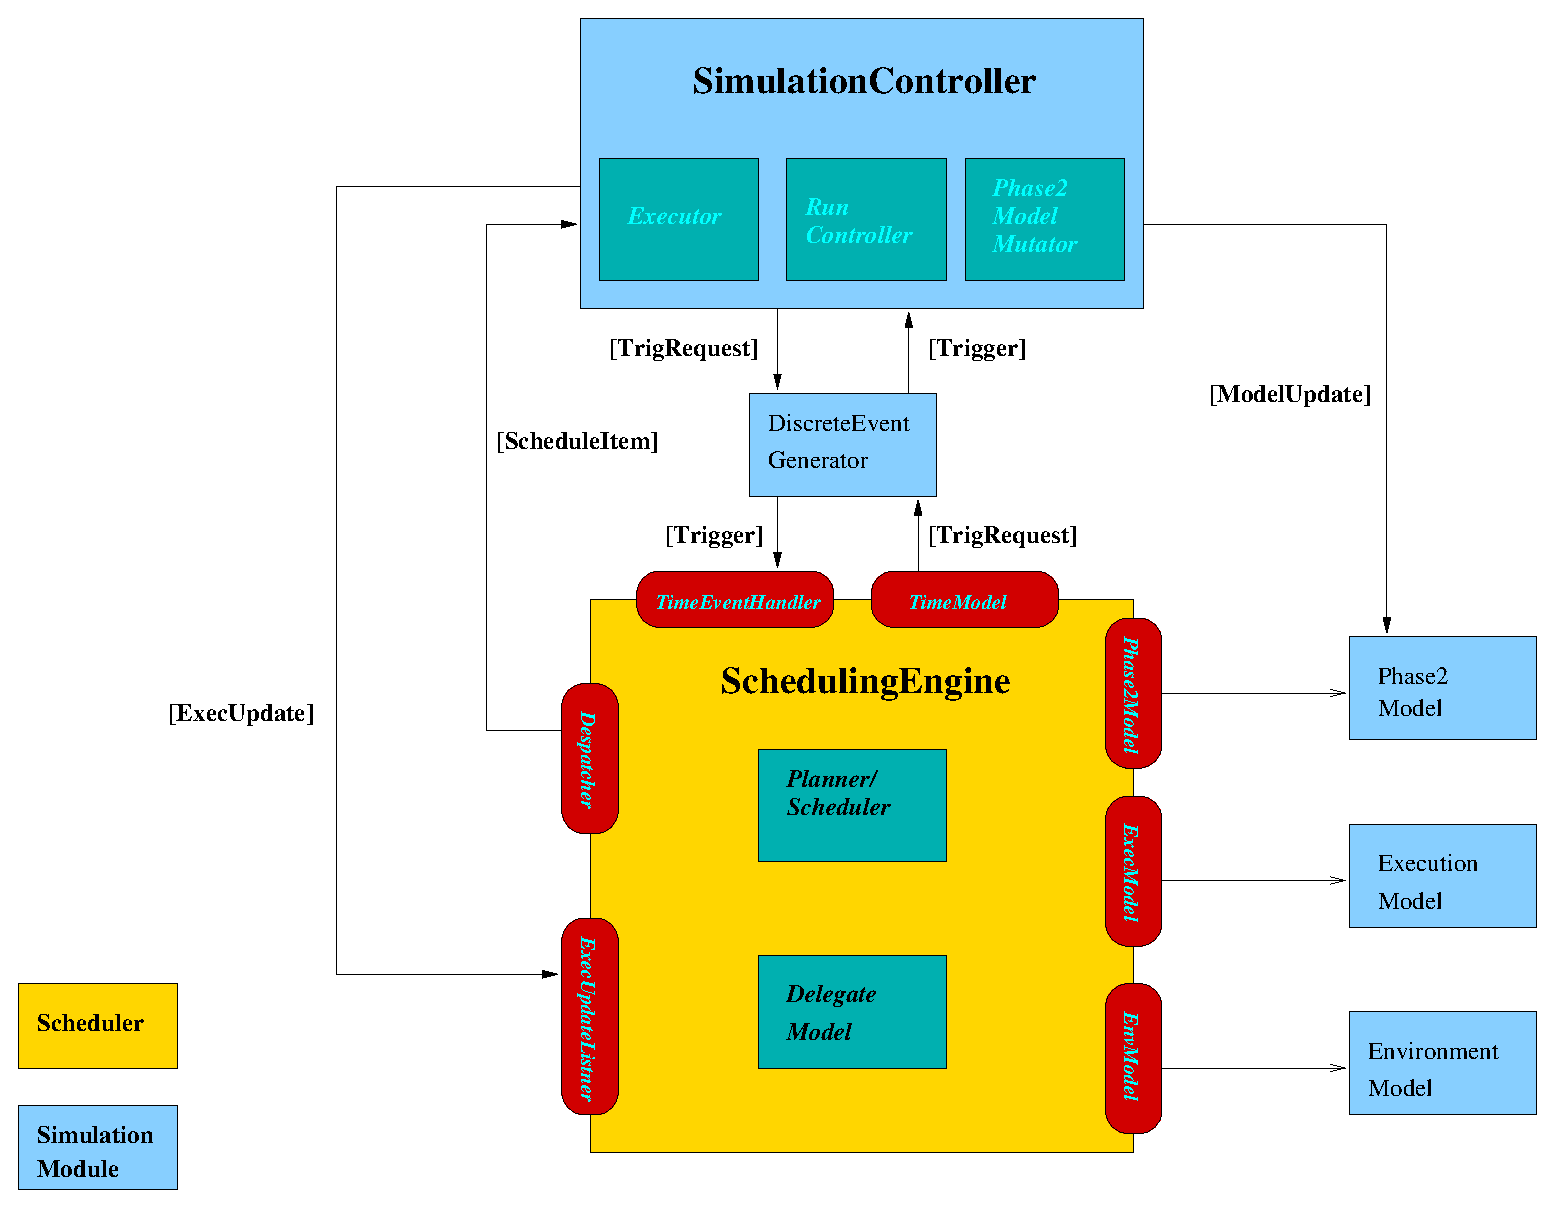
\includegraphics[height=6cm]{figures/sim_framework.eps}
%   \end{center}
%   \label{fig:simframewrk} 
%   \caption[Scheduling simulation framework.] 
%   {Architecture of scheduling simulation framework.}
%   \end{figure} 


\begin{landscape}
   \begin{figure}[htp]
   \begin{center}
   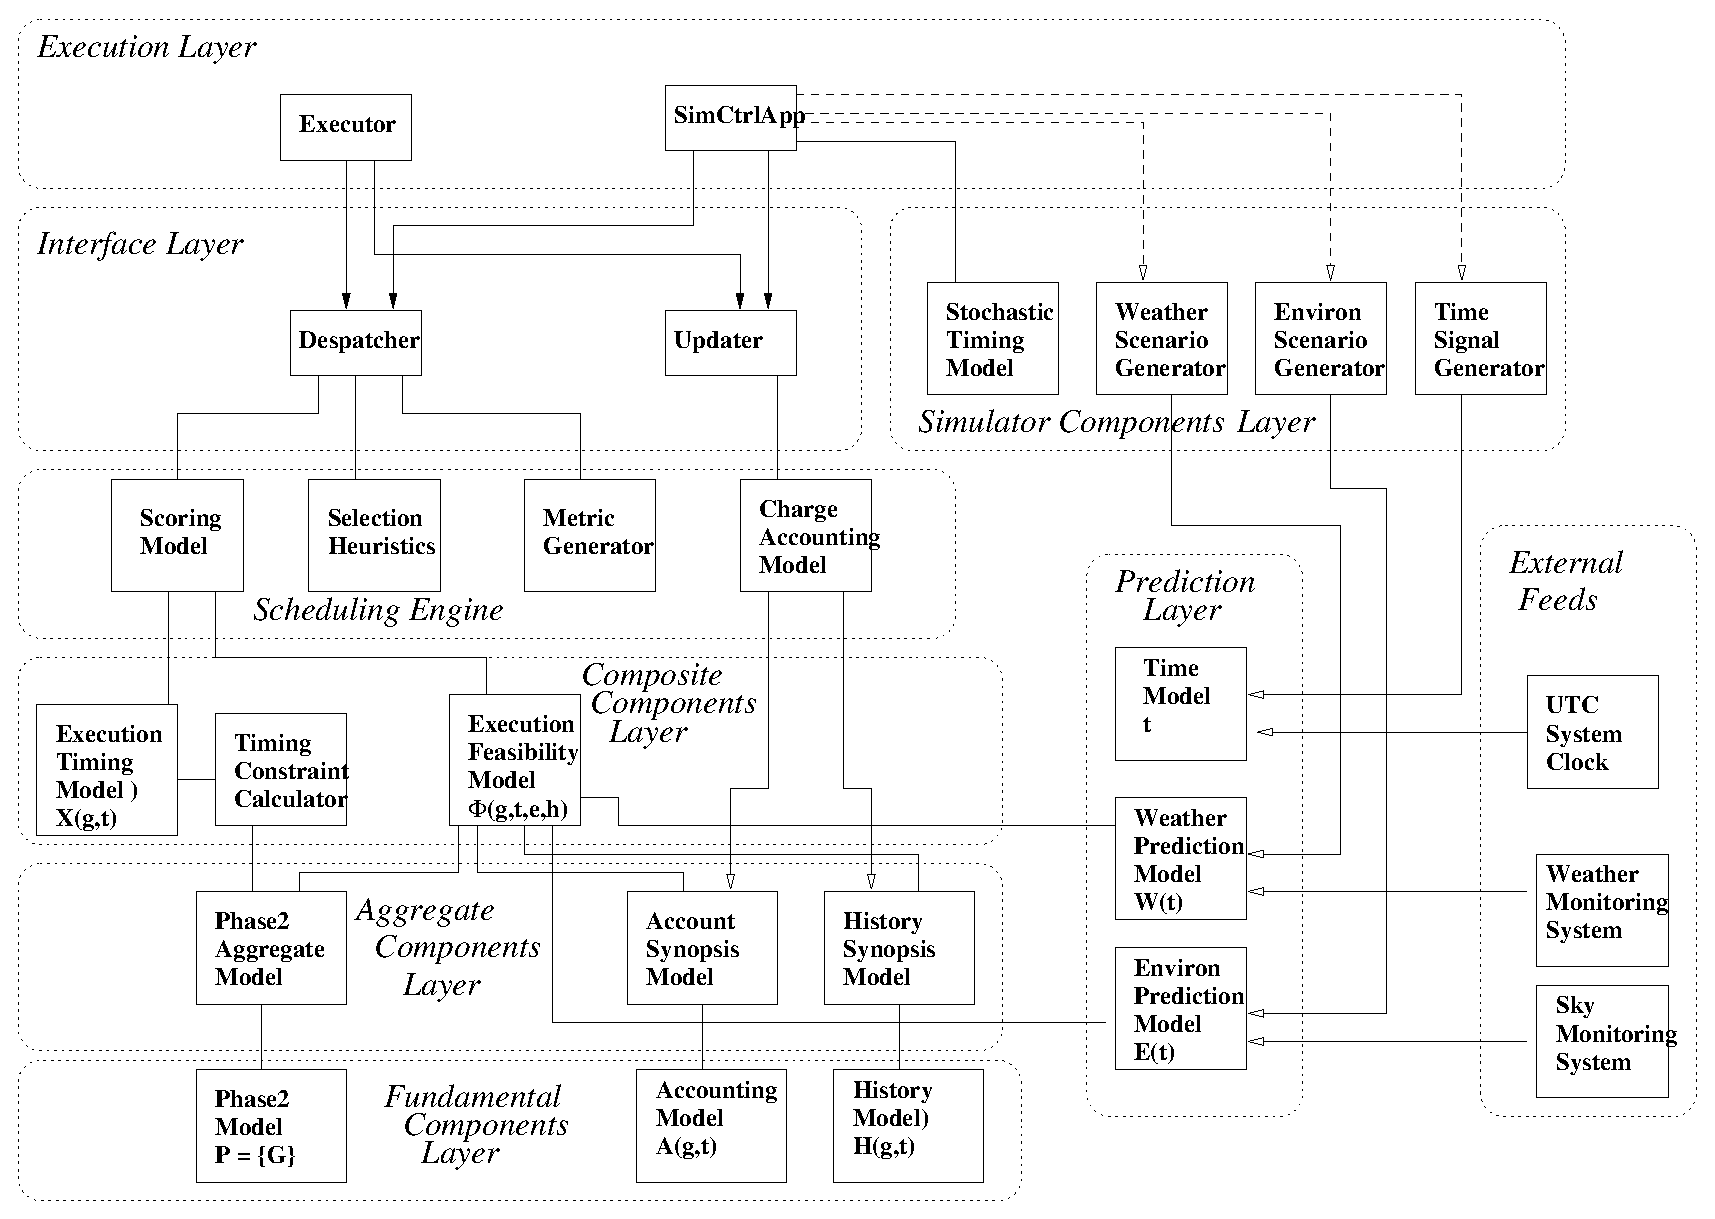
\includegraphics[height=14cm]{figures/sca.eps}
   \end{center}
   \label{fig:simframewrk} 
   \caption[Scheduling simulation framework.] 
   {Architecture of scheduling simulation framework.}
   \end{figure} 
\end{landscape}

Whats going on here ? The sim controller provides all the models for the SE - The EnvModel is likely generated on-the-fly based on current time and some provided function (or e.g. random variation about some mean level or with some trend...). The ExecModel likely uses a random variation


Some details about a test of different bias functions.
Effect of snapshot age on calculations - especially wrt (Problem Quality Metrics) PQMs.

What are the effects of various simulation assumptions ? Namely effects like phase2 drift. I will run a series of experments to test the effect of length of lookahead - this can be done using the following method:-
work out demand profile d(t) for N nights ahead. Run simulation for 1 night and recalculate - now for N-1 nights ahead, keep doing this so on step r we simulate night r and work out d(t) for N-r nights ahead. Variation on this could include the effects of varying the Env model. Basically I just want to know if look ahead calculation of D(t) works - can also compare this to working out D(t) for r using different ODB snapshots.

This was the FWDDMD set of results - add graphs here XXX. Notes: ODB snapshot 31oct07, run for 3x days ahead. Using scoring model $S_{xxx}$ - need to get from standard SCO model table in scoremodel section

\subsection{Additional simulator components}

\subsubsection{Stochastic Execution Timing Model - $\xi$}
This represents the execution environment's model of timing...

Figure \ref{fig:simf_exec_timing_dist} shows examples of the distribution of execution times derived for a single group calculated 100000 times. The two plots show the effect of different assumptions on the contributions of seperate random timing events. The group consisting 12x30s exposures with 3 config changes and 3 target changes (slews).

\begin{figure}[h]
\begin{center}
 \label{fig:simf_exec_timing_dist}
  \includegraphics[height=6cm, angle=-90]{figures/simf_exec_plot.eps}
\caption[Distribution of execution times for stochastic execution model]
{Distribution of execution times for stochastic execution model. \emph{Mono} plot uses a single calculation to total up contribution of all events, \emph{multi} plot works out a seperate random effect for each contributing event}
\end{center}
\end{figure}

\subsubsection{Environmental Scenario ($\sum$)}
This allows an environment (sky conditions) scenario to be represented. It can be taken from actual processed sky conditions data or generated by an Environmental Scenario Generator (ESG). We are not usually bothered about the actual details just the general classification of conditions into extinction as photometric/non-photometric and seeing into one of the 3 or 4 pre-defined bands.


\subsubsection{Weather scenario ($\Omega$)}
This allows a weather scenario to be represented. It can be taken from actual processed weather data or generated by a weather Scenario Generator (WSG). As with environmental scenario we only need to know if the weather is good or bad not the details though this level of detail may be needed for prediction modelling.

\subsubsection{Quality/Complexity metric plugins}
Various plugins to measure schedule quality and problem complexity to suit the application.

\subsubsection{Time signal generator}
In conjunction with timing event listener handles synchronization between scheduler and executor components. This is relevant for situations where XM and SM are indeed running in parallel - big problem is where SM takes a finite time to perform some operation that XM just jumps time forward.
